\section{Multi-threaded processors}
    Arithmetic units in CPUs are often not busy because there is long-latency memory accesses, exceptions due to I/O or syscalls, etc\ldots Then, we often switch threads a lot. The thing is, can we keep thread context around in hardware instead of save and restore context every time?\\

    Let's remind how looks a basic superscalar pipeline:
    \begin{center}
        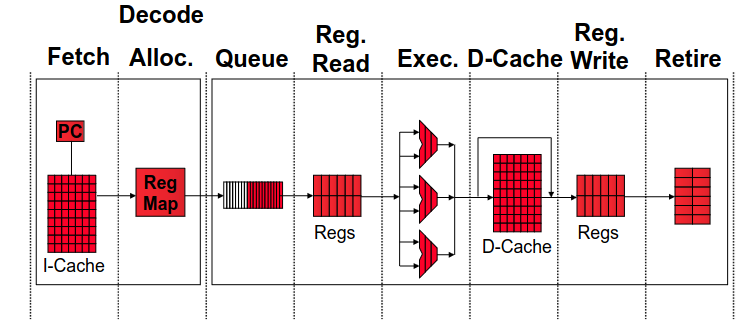
\includegraphics[width=9cm]{images/74.png} 
    \end{center}
    Pipelining allows multiple instructions to be in-flight:

    \begin{image}{Assuming 5 stages (F, D, X, M, W) and a perfect 

        pipeline \textrightarrow \space scalar IPC = 1.

    On superscalar, we can duplicate the pipeline \textrightarrow IPC = 2.}
    \begin{center}
        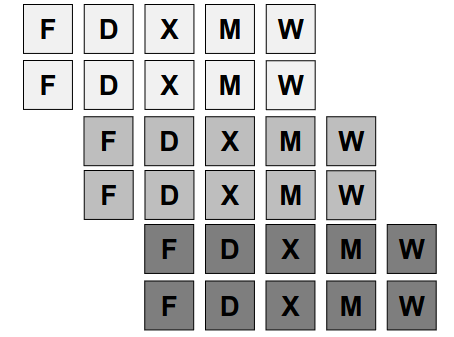
\includegraphics[width=5cm]{images/75.png} 
    \end{center}
    \end{image}
    \begin{tcolorbox}[vert]
    But, in reality, there can be pipeline bubbles that decrease IPC. They can occurs for multiple reason, one is \important{structural hazards}: not enough resources are available and instructions are queued, waiting for resources to free up.

    For example, in a 2-way in-order superscalar processor with one cache port (or one load or store per cycle), if two loads align in same cycle, second one must wait.
    \end{tcolorbox}
    \begin{image}{If we take the same setup we can see this in this code for example:}
     \begin{codeCenter}
    \begin{Ccode}
for (i =0; i < N; i++)
    a[i] += (b[i] + c[i])
    \end{Ccode}
    \end{codeCenter}
    \end{image}
    
       \begin{image}{That would look like this in 

        assembly:}
    \begin{codeCenter}
    \begin{Ccode}
loop:
    lw r5 , 0(r2)
    lw r6 , 0(r3)
    lw r7 , 0(r4)
    add r5 , r5 , r6
    add r5 , r5 , r7
    sw r5 , 0(r2)
    addi r2 , r2 , 4
    addi r3 , r3 , 4
    sub r9, r8, r2 ;
    addi r4 , r4 , 4
    bne r9, loop
    \end{Ccode}
    \end{codeCenter}
    \end{image}
       Then, because we have only one cache port, we would have bubble on the load operations:
    \begin{center}
        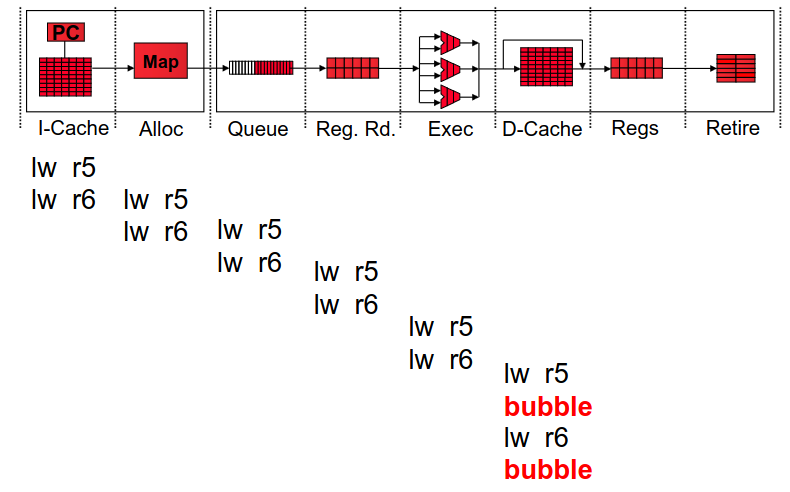
\includegraphics[width=8cm]{images/76.png} 
    \end{center}
    And our pipeline would have bubbles (also caused by the add waiting for \texttt{sw} operation):
    \begin{center}
        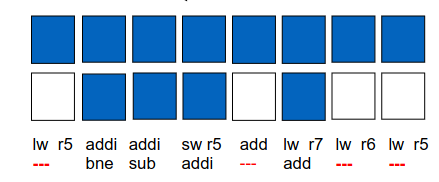
\includegraphics[width=7cm]{images/77.png} 
    \end{center}
    Finally we obtain an average IPC of 1.6 ($\frac{\#\text{ instrs}}{\# \text{ cycles}}=\frac{11}{7}=1.6$).
    \begin{tcolorbox}[vert]
        An other reason why pipeline bubbles occurs is the \important{branch control flow}: it's when we predict the branch direction to keep fetching instructions.

    If we are waiting for the real direction before fetching it would introduces bubbles: two cycles minimum with a shallow pipeline because we usually know the target of the branch (e.g. \texttt{beq}) on the execute stage. Real pipelines are much deeper (14+) so we prefer to predict the target of the branch to continue to fetch immediately. If the prediction was right we continue, otherwise we flush the pipeline.
    \end{tcolorbox}
    Finally data dependencies can also obviously create bubbles in the pipeline: they can't execute in the same cycle, etc\ldots But we remember that with OoO cores, we can easily traverses loops and issues loads.
    \begin{tcolorbox}[rouge]
        But real programs are not so simple: there is many cycles where nothing can be issued a more realistic IPC would be between 0.5 and 1.
    \end{tcolorbox}
    \begin{tcolorbox}[vert]
    We can imagine then that there is a lot of waste, we classify it in two categories:
    \begin{itemize}[left=10pt, label=\textbullet]
        \item \important{Vertical waste}: whole cycle is empty, nothing issued, this is common after long latency events.
        \item \important{Horizontal waste}: we are unable to use full issue width, this is when the software isn't exposing enough ILP for hardware (the code isn't enough parallelizable).
    \end{itemize}
    \end{tcolorbox}
    \begin{center}
        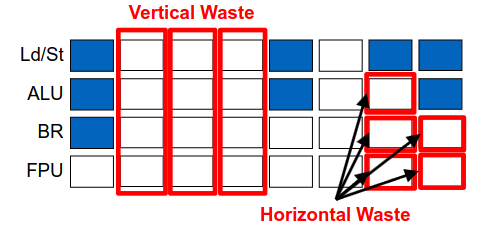
\includegraphics[width=8cm]{images/78.png} 
    \end{center}
    \begin{tcolorbox}[vert]
        To solve this, the idea of \important{hardware multithreading} is to find ready instructions from many threads. But it requires to have thread context (PC, SP, register file, interrupt descriptors) in hardware.
    \end{tcolorbox}
    So we said that we have to store the context, so it has a hardware cost: each thread needs architectural state with a register, the PC, the stack and the interrupt tables. It costs SRAM and can impact area especially for small cores.

    Threads are also sharing the memory hierarchy now:
    \begin{itemize}[left=10pt, label=\textbullet]
        \item It causes potential contention in the data cache, 
        \item It causes contention in instruction cache, 
        \item It will affect single thread performance (better throughput but worse latency).
    \end{itemize}
    \newpage
    \subsection{CGMT vs. FGMT}
        
    \begin{tcolorbox}[vert]
    The \important{coarse grained multithreading implementation (CGMT)} consist in switching to a new thread on a long latency event.
    \end{tcolorbox}
    \begin{center}
        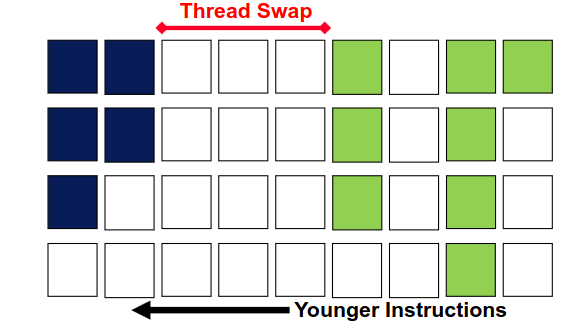
\includegraphics[width=6cm]{images/79.png} 
    \end{center}
    \begin{remark}{Remark}
        We can see that the real difference of hardware multithreading with user-level/OS context switching is that it takes only few cycles instead of multiple milliseconds.
    \end{remark}
    If we made the choice of not having a 4-way pipeline with hardware multithreading but two cores with 2-way pipeline, it would have less horizontal waste but it would suffer from more vertical on long latency.
    \begin{center}
        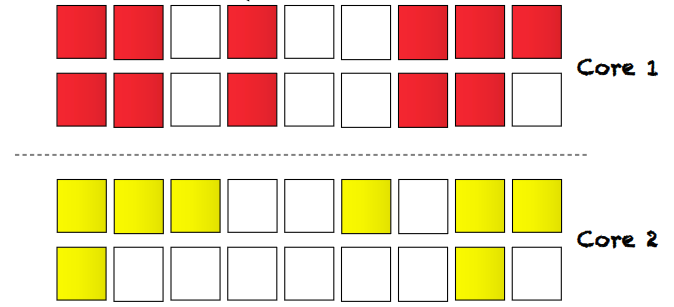
\includegraphics[width=6cm]{images/80.png} 
    \end{center}
    \begin{tcolorbox}[violet]
    The critical decision on CGMT is when we have to switch threads: the thread switch + the pipe fill time should be way smaller that the blocking latency.\\

    The advantage of CGMT is that it requires small changes to existing hardware but it slow down the performance of a single-thread (shared resources, etc\ldots).
    \end{tcolorbox}
    \begin{tcolorbox}[vert]
        The \important{fine grained multithreading implementation (FGMT)} consist in cycle between multiple threads periodically, we eliminate the switch time by keeping all thread hot.
    \end{tcolorbox}
    \begin{center}
        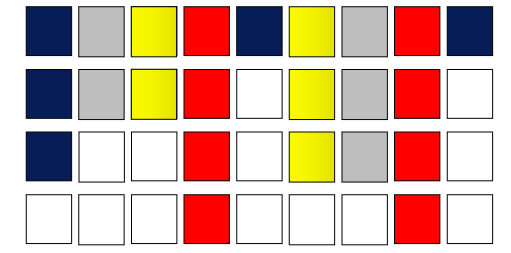
\includegraphics[width=5cm]{images/81.png} 
    \end{center}
    If we compare both CGMT and FGMT it looks respectfully like this:
    \begin{center}
    \begin{minipage}{0.45\textwidth}
            \begin{center}
        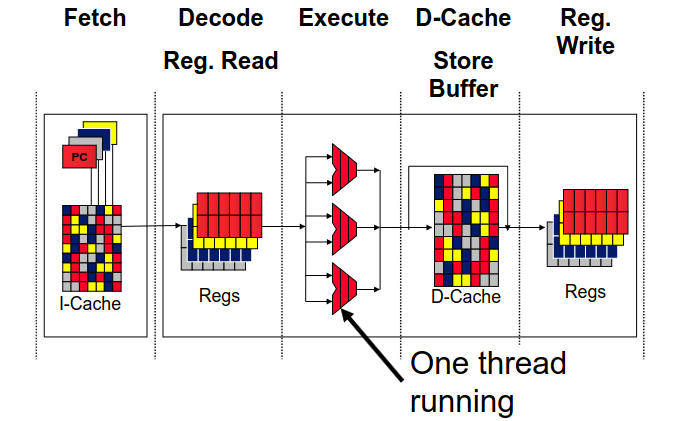
\includegraphics[width=7cm]{images/82.png} 
            \end{center}
    \end{minipage}
    \hfill
    \begin{minipage}{0.45\textwidth}
       \begin{center}
        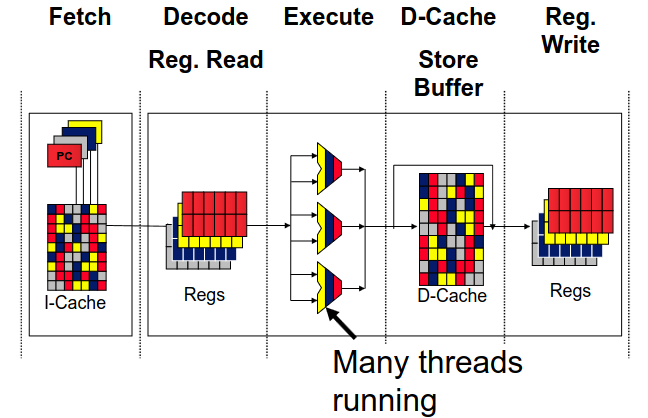
\includegraphics[width=7cm]{images/83.png}
        \end{center}
    \end{minipage}
    \end{center}
    In FGMT design there is no critical decision, to improve throughput we only have to have enough threads to eliminate vertical waste (e.g. for a pipeline depth of 8, using 8 threads isn't enough).\\

    FGMT have a reasonable single thread performance and is efficient in case of many thread. But it's more complicated for hardware to track dependencies and many more contexts means we need many more registers.

    Notify that both, CGMT and FGMT cannot address horizontal waste, only vertical.
    \subsection{SMT}
        \begin{tcolorbox}[vert]
            The idea of \important{simultaneous multithreading (SMT)} is to have instructions from multiple threads in the same cycle. This is the first design that can reduce horizontal waste.
        \end{tcolorbox}
        \begin{center}
        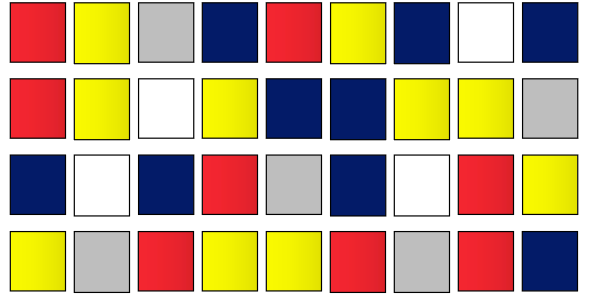
\includegraphics[width=5cm]{images/84.png}
        \end{center}
        Previously, only caches and predictors were shared, with SMT, instructions from different threads are interleaved in the same cycle.

        But do we need then to resolve all potential dependencies between threads (e.g. $T_1$ and $T_2$ are both executing \texttt{add r1, r2, r3})? No we don't because registers are physically mapped then,
        \[T_1: \text{\texttt{add r1, r2, r3} becomes: \texttt{add p4, p2, p3}}\]
        \[T_2: \text{\texttt{add r1, r2, r3} becomes: \texttt{add p9, p8, p5}}\]
        \begin{tcolorbox}[rouge]
        After instruction allocation, the scheduler becomes thread-agnostic, meaning it no longer distinguishes between different threads and only sees independent micro-operations.\\
        
            Some pipeline stages must still maintain per-thread state. In particular, the Fetch, Decode, and Allocate (register renaming) stages are duplicated for each thread. Each thread has its own program counter and its own register mapping table, which ensures correct tracking of architectural registers during renaming. Retire (commit) stage must also know its thread identity, since it is responsible for committing instructions in order and freeing the correct physical registers associated with each thread.\\
            
    There are two main strategies for sharing pipeline structures in SMT systems.
    \begin{itemize}[left=10pt, label=\textbullet]
        \item The first is static partitioning, where each thread is assigned a fixed portion of the hardware resources.
        \item The other is dynamic sharing, it means all threads use the same hardware resources, with each entry tagged to indicate which thread it belongs to.
    \end{itemize}
        \end{tcolorbox}
        The implementation look then like this:
        \begin{center}
        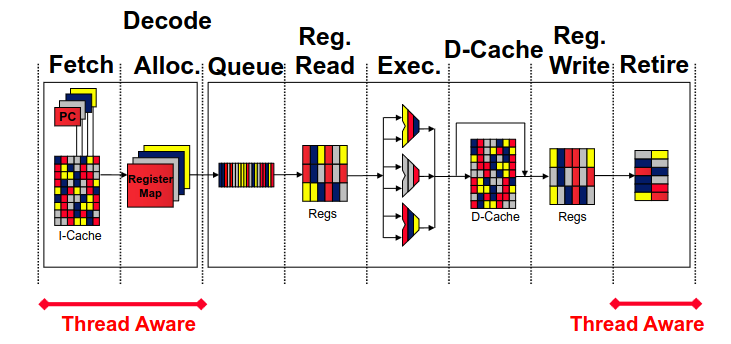
\includegraphics[width=10cm]{images/85.png}
        \end{center}
    The critical decision for SMT is the fetch-interleaving policy: since multiple threads are active, the processor must choose which thread provide instructions to the pipeline at any given time.\\

    The requirement to improve throughput is that we should have enough threads to utilize resources but fewer than needed to stretch dependencies.
    \begin{tcolorbox}[gris]
        So how to decide which threads fetch instructions? The goal is to maximize active use of issue width. \\
        
            ICOUNT is the common policy: threads with fewest instructions in pipe has priority. ICOUNT does not need to know why a thread is stalled, It just observes: ``this thread has fewer active instructions in the pipeline \textrightarrow \space it is more stalled''.
    \end{tcolorbox}
    SMT performs well when threads do not interfere with each other’s state in shared structures such as caches, branch predictors, and the ROB. It requires sufficient hardware resources to be effective; otherwise, extra thread context cannot be exploited.

    It is especially well suited to wide-issue out-of-order processors, where unused execution slots can be filled by other threads.

    \begin{remark}{Remark}
        Private caches for SMT are easier to implement but shared caches are faster to communicate among threads, there is no coherence overhead and offers more flexibility in allocating resources.
    \end{remark}
